\documentclass{article}

% content/resources/templates/preamble.tex
\usepackage[margin=0.6in]{geometry}
\author{Milav Dabgar}
\usepackage{amsmath,amssymb,amsthm}
\usepackage{booktabs}
\usepackage{multirow}
\usepackage{xcolor}
\usepackage{tcolorbox}
\tcbuselibrary{breakable,skins}
\usepackage[colorlinks=true,linkcolor=blue]{hyperref}
\usepackage{titlesec}
\usepackage{enumitem}
\usepackage{tikz}
\usepackage{pgfplots}
\usepackage{circuitikz}
\usepackage[version=4]{mhchem}
\usepackage{longtable}
\usepackage{array}
\usepackage{float}
\usepackage{caption}
\usepackage{listings}

\lstset{
  basicstyle=\small\ttfamily,
  breaklines=true,
  breakatwhitespace=false,
  postbreak=\mbox{\textcolor{red}{$\hookrightarrow$}\space},
  float=false,
  numbers=left,
  numberstyle=\tiny\color{gray},
  numbersep=10pt,
  xleftmargin=2em,
  keywordstyle=\color{blue},
  commentstyle=\color{green!60!black},
  stringstyle=\color{purple},
  backgroundcolor=\color{gray!5},
  showstringspaces=false,
  tabsize=2,
  captionpos=b,
  keepspaces=true,
  columns=flexible
}

\pgfplotsset{compat=1.18}
\usetikzlibrary{shapes,arrows,positioning,calc,patterns,decorations.pathmorphing,decorations.markings,arrows.meta}

% Color scheme
\definecolor{headcolor}{RGB}{0,102,204}
\definecolor{keycolor}{RGB}{220,20,60}
\definecolor{solutioncolor}{RGB}{34,139,34}
\definecolor{mnemoniccolor}{RGB}{148,0,211}
\definecolor{codecolor}{RGB}{0,0,100}

% Spacing
\setlength{\parskip}{3pt}
\setlist[itemize]{nosep}
\setlist[enumerate]{nosep}

% Title formatting
\titleformat{\section}{\Large\bfseries\color{headcolor}}{\thesection}{1em}{}
\titleformat{\subsection}{\large\bfseries\color{headcolor}}{\thesubsection}{1em}{}

% Pandoc tightlist compatibility
\providecommand{\tightlist}{%
  \setlength{\itemsep}{0pt}\setlength{\parskip}{0pt}}

% Pandoc longtable compatibility
\newcounter{none}
\def\thenone{}


% content/resources/templates/english-boxes.tex

% Custom environments
\newtcolorbox{solutionbox}{
 breakable,
 enhanced,
 colback=solutioncolor!5!white,
 colframe=solutioncolor!75!black,
 fonttitle=\bfseries,
 title=Solution
}

\newtcolorbox{solutionboxnobreak}{
 colback=solutioncolor!5!white,
 colframe=solutioncolor!75!black,
 fonttitle=\bfseries,
 title=Solution
}

\newtcolorbox{keyformula}{
 breakable,
 enhanced,
 colback=keycolor!5!white,
 colframe=keycolor!75!black,
 fonttitle=\bfseries,
 title=Key Formula
}

\newtcolorbox{mnemonicboxenv}{
 breakable,
 enhanced,
 colback=mnemoniccolor!5!white,
 colframe=mnemoniccolor!75!black,
 fonttitle=\bfseries,
 title=Mnemonic
}

\newcommand{\mnemonicbox}[1]{%
  \begin{mnemonicboxenv}
    #1
  \end{mnemonicboxenv}
}


% Custom commands for GTU solutions
% This file defines semantic commands for consistent formatting

% Question command with automatic formatting
\newcommand{\question}[2]{%
  \section*{Question #1}%
  \textbf{#2}%
}

% OR question variant
\newcommand{\questionor}[2]{%
  \section*{Question #1 OR}%
  \textbf{#2}%
}

% Proper table environment with caption
\newenvironment{answertable}[1]{%
  \begin{table}[htbp]
  \centering
  \caption{#1}
}{%
  \end{table}
}

% Proper figure environment for diagrams
\newenvironment{answerdiagram}[1]{%
  \begin{figure}[htbp]
  \centering
  \caption{#1}
}{%
  \end{figure}
}

% Semantic markup for key terms
\newcommand{\keyword}[1]{\textbf{#1}}
\newcommand{\code}[1]{\texttt{#1}}
\newcommand{\classname}[1]{\texttt{#1}}
\newcommand{\methodname}[1]{\texttt{#1}}

% Proper quotation marks
\newcommand{\mnemonic}[1]{``#1''}


\title{Mathematics (4300001) - Winter 2022 Solution}
\date{February 24, 2023}

\begin{document}
\maketitle

\questionmarks{1}{14}{Fill in the blanks using appropriate choice from the given options}

\questionmarks{1.1}{1}{If $\begin{vmatrix} x & 8 \\ 2 & 4 \end{vmatrix} = 0$ then the value of $x$ is \_\_\_\_}
\begin{solutionbox}
\textbf{Answer}: a. 4

\textbf{Solution}:
\[ \begin{vmatrix} x & 8 \\ 2 & 4 \end{vmatrix} = x(4) - 8(2) = 4x - 16 \]

Given: $4x - 16 = 0 \implies 4x = 16 \implies x = 4$
\end{solutionbox}

\questionmarks{1.2}{1}{$\begin{vmatrix} 2 & -9 & 1 \\ 5 & -8 & 4 \\ 0 & 3 & 0 \end{vmatrix} = $ \_\_\_\_}
\begin{solutionbox}
\textbf{Answer}: a. -9

\textbf{Solution}:
Expanding along the third row:
\[ = 0 - 3 \begin{vmatrix} 2 & 1 \\ 5 & 4 \end{vmatrix} + 0 \]
\[ = -3(2 \times 4 - 1 \times 5) = -3(8 - 5) = -3(3) = -9 \]
\end{solutionbox}

\questionmarks{1.3}{1}{If $f(x) = \log x$ then $f(1) = $ \_\_\_\_}
\begin{solutionbox}
\textbf{Answer}: a. 0

\textbf{Solution}:
$f(x) = \log x \implies f(1) = \log 1 = 0$
\end{solutionbox}

\questionmarks{1.4}{1}{$\log x + \log(\frac{1}{x}) = $ \_\_\_\_}
\begin{solutionbox}
\textbf{Answer}: a. 0

\textbf{Solution}:
$\log x + \log(\frac{1}{x}) = \log x + \log x^{-1} = \log x - \log x = 0$
\end{solutionbox}

\questionmarks{1.5}{1}{$120^\circ = $ \_\_\_\_\_ radian}
\begin{solutionbox}
\textbf{Answer}: b. $\frac{2\pi}{3}$

\textbf{Solution}:
$120^\circ = 120 \times \frac{\pi}{180} = \frac{120\pi}{180} = \frac{2\pi}{3}$ radians
\end{solutionbox}

\questionmarks{1.6}{1}{$\sin^{-1}(\sin \frac{\pi}{6}) = $ \_\_\_\_\_}
\begin{solutionbox}
\textbf{Answer}: c. $\frac{\pi}{6}$

\textbf{Solution}:
Since $\frac{\pi}{6} \in [-\frac{\pi}{2}, \frac{\pi}{2}]$, $\sin^{-1}(\sin \frac{\pi}{6}) = \frac{\pi}{6}$
\end{solutionbox}

\questionmarks{1.7}{1}{The principal period of $\tan \theta$ is \_\_\_\_\_}
\begin{solutionbox}
\textbf{Answer}: b. $\pi$

\textbf{Solution}:
The principal period of $\tan \theta$ is $\pi$.
\end{solutionbox}

\questionmarks{1.8}{1}{$|2i - j + 2k| = $ \_\_\_\_}
\begin{solutionbox}
\textbf{Answer}: a. 3

\textbf{Solution}:
$|2i - j + 2k| = \sqrt{2^2 + (-1)^2 + 2^2} = \sqrt{4 + 1 + 4} = \sqrt{9} = 3$
\end{solutionbox}

\questionmarks{1.9}{1}{$i \cdot i = $ \_\_\_\_}
\begin{solutionbox}
\textbf{Answer}: a. 1

\textbf{Solution}:
$i \cdot i = |i|^2 = 1^2 = 1$
\end{solutionbox}

\questionmarks{1.10}{1}{The slope of line $x - 4 = 0$ is \_\_\_\_\_\_}
\begin{solutionbox}
\textbf{Answer}: d. Not Defined

\textbf{Solution}:
Line $x = 4$ is a vertical line. Its slope is undefined.
\end{solutionbox}

\questionmarks{1.11}{1}{The center of circle $x^2 + y^2 = 4$ is}
\begin{solutionbox}
\textbf{Answer}: c. $(0,0)$

\textbf{Solution}:
Comparing with $(x - h)^2 + (y - k)^2 = r^2$:
Center is $(0, 0)$.
\end{solutionbox}

\questionmarks{1.12}{1}{$\lim_{x \to 2} \frac{x^4 - 16}{x - 2} = $ \_\_\_\_}
\begin{solutionbox}
\textbf{Answer}: c. 32

\textbf{Solution}:
Using form $\lim_{x \to a} \frac{x^n - a^n}{x - a} = na^{n-1}$:
$= 4 \times 2^{4-1} = 4 \times 2^3 = 4 \times 8 = 32$
\end{solutionbox}

\questionmarks{1.13}{1}{$\lim_{n \to 0} (1 + n)^{\frac{1}{n}} = $ \_\_\_\_}
\begin{solutionbox}
\textbf{Answer}: d. $e$

\textbf{Solution}:
Definition of $e$: $\lim_{n \to 0} (1 + n)^{\frac{1}{n}} = e$
\end{solutionbox}

\questionmarks{1.14}{1}{$\lim_{x \to 0} \frac{\sin 6x}{3x} = $ \_\_\_\_}
\begin{solutionbox}
\textbf{Answer}: c. 2

\textbf{Solution}:
$\lim_{x \to 0} \frac{\sin 6x}{6x} \times 2 = 1 \times 2 = 2$
\end{solutionbox}

\questionmarks{2(A)}{6}{Attempt any two}

\questionmarks{2.1}{3}{If $\begin{vmatrix} 2 & 6 & 4 \\ -1 & x & 0 \\ 5 & 9 & -2 \end{vmatrix} = 0$ then find $x$}
\begin{solutionbox}
\textbf{Solution}:
Expanding along the second row:
\[ \begin{vmatrix} 2 & 6 & 4 \\ -1 & x & 0 \\ 5 & 9 & -2 \end{vmatrix} = -(-1) \begin{vmatrix} 6 & 4 \\ 9 & -2 \end{vmatrix} + x \begin{vmatrix} 2 & 4 \\ 5 & -2 \end{vmatrix} - 0 \]
Wait, expanding along R2 signs are $-, +, -$.
Term 1: $-(-1) |...| = 1(6(-2) - 36) = -12 - 36 = -48$
Term 2: $+x(2(-2) - 20) = x(-4 - 20) = -24x$

So, $-48 - 24x = 0 \implies 24x = -48 \implies x = -2$.

\textit{Re-checking calculation from MDX solution steps:}
MDX solution says:
$= 1(-12 - 36) - x(-4 - 20)$ (Wait, MDX had $-x$ for middle term??)
MDX text: "Expanding along the second row... -(-1)... -x...".
Actually sign pattern for determinant is:
+ - +
- + -
+ - +
So for second row: $-(-1)$, $+x$, $-0$.
So it should be $+1(\dots) + x(\dots) - 0$.
Calculation:
$1(6(-2) - 4(9)) = 1(-12 - 36) = -48$.
$x(2(-2) - 4(5)) = x(-4 - 20) = -24x$.
Sum: $-48 - 24x = 0 \implies x = -2$.

Let's check MDX solution result again.
MDX Solution:
$= 1(-12 - 36) - x(-4 - 20)$ <- This line has a sign error for $x$ term if standard expansion. BUT $x$ is at (2,2) position, so sign is positive. EXCEPT if they expanded differently.
MDX result: $x = 2$.
Let's re-eval:
If $x=2$:
$\begin{vmatrix} 2 & 6 & 4 \\ -1 & 2 & 0 \\ 5 & 9 & -2 \end{vmatrix}$
R3: $5(0-8) - 9(0+4) + (-2)(4+6) = -40 - 36 - 20 \neq 0$.
So $x=2$ is likely WRONG.

Let's check $x=-2$:
$\begin{vmatrix} 2 & 6 & 4 \\ -1 & -2 & 0 \\ 5 & 9 & -2 \end{vmatrix}$
R3 expansion: $5(0 - (-8)) - 9(0 - (-4)) + (-2)(-4 - (-6))$
$= 5(8) - 9(4) - 2(2) = 40 - 36 - 4 = 0$.
So correct answer is $x = -2$.

\textbf{Correction Note}: The MDX solution derives $x=2$ but verification shows $x=-2$. I will provide the mathematically correct derivation yielding $x=-2$.

Correct Expansion along R2:
Element $a_{21} = -1$ (Sign -): $-(-1) \begin{vmatrix} 6 & 4 \\ 9 & -2 \end{vmatrix} = 1(-12 - 36) = -48$
Element $a_{22} = x$ (Sign +): $+x \begin{vmatrix} 2 & 4 \\ 5 & -2 \end{vmatrix} = x(-4 - 20) = -24x$
Element $a_{23} = 0$: 0

Total: $-48 - 24x = 0 \implies -24x = 48 \implies x = -2$.
So result is $x = -2$.
\end{solutionbox}

\questionmarks{2.2}{3}{If $f(x) = \tan x$ then prove that (i) $f(x+y) = \frac{f(x) + f(y)}{1 - f(x)f(y)}$, (ii) $f(2x) = \frac{2f(x)}{1 - [f(x)]^2}$}
\begin{solutionbox}
\textbf{Solution}:
Given: $f(x) = \tan x$

(i) To prove $f(x+y) = \frac{f(x) + f(y)}{1 - f(x)f(y)}$:
LHS $= f(x+y) = \tan(x+y)$
Using tangent addition formula:
\[ \tan(x+y) = \frac{\tan x + \tan y}{1 - \tan x \tan y} \]
Substituting $f(x) = \tan x$ and $f(y) = \tan y$:
\[ = \frac{f(x) + f(y)}{1 - f(x)f(y)} = \text{RHS} \]

(ii) To prove $f(2x) = \frac{2f(x)}{1 - [f(x)]^2}$:
LHS $= f(2x) = \tan(2x)$
Using double angle formula:
\[ \tan(2x) = \frac{2\tan x}{1 - \tan^2 x} \]
\[ = \frac{2f(x)}{1 - [f(x)]^2} = \text{RHS} \]
\end{solutionbox}

\questionmarks{2.3}{3}{Prove that $\frac{\sin 3A - \cos 3A}{\sin A - \cos A} = 2$}
\begin{solutionbox}
\textbf{Solution}:
Identities:
$\sin 3A = 3\sin A - 4\sin^3 A$
$\cos 3A = 4\cos^3 A - 3\cos A$

LHS $= \frac{(3\sin A - 4\sin^3 A) - (4\cos^3 A - 3\cos A)}{\sin A - \cos A}$
\[ = \frac{3(\sin A + \cos A) - 4(\sin^3 A + \cos^3 A)}{\sin A - \cos A} \]

Using $a^3 + b^3 = (a+b)(a^2 - ab + b^2)$:
$\sin^3 A + \cos^3 A = (\sin A + \cos A)(1 - \sin A \cos A)$

Numerator becomes:
\[ (\sin A + \cos A) [3 - 4(1 - \sin A \cos A)] \]
\[ = (\sin A + \cos A) [3 - 4 + 4\sin A \cos A] \]
\[ = (\sin A + \cos A) [ -1 + 4\sin A \cos A ] \]

Divide by $(\sin A - \cos A)$...
Wait, let's check the question again.
Usually $\frac{\sin 3A}{\sin A} - \frac{\cos 3A}{\cos A} = 2$.
Is it possible the question is typed wrong in MDX?
Let's check values. Let $A = 30^\circ$.
$\frac{\sin 90 - \cos 90}{\sin 30 - \cos 30} = \frac{1 - 0}{0.5 - 0.866} = \frac{1}{-0.366} \approx -2.7 \neq 2$.
Let's check $A=45^\circ$.
Denominator 0. Undefined.

Maybe the question is $\frac{\cos 3A}{\cos A} + \frac{\sin 3A}{\sin A}$? No.
Maybe $\frac{\sin 3A + \sin^3 A}{\dots}$.

Let's look at the MDX solution again.
"After further simplification using trigonometric identities, this equals 2."
It skips the derivation.
Let's check if the expression simplifies.
Numerator: $(\sin A + \cos A)(4\sin A \cos A - 1)$.
Denominator: $\sin A - \cos A$.
This does not divide nicely to give 2.

Hypothesis: Question is actually $\frac{\sin 3A}{\sin A} - \frac{\cos 3A}{\cos A} = 2$.
LHS $= (3 - 4\sin^2 A) - (4\cos^2 A - 3) = 6 - 4(\sin^2 A + \cos^2 A) = 6 - 4 = 2$.
This fits perfectly.
The MDX text has "$\frac{\sin 3A - \cos 3A}{\sin A - \cos A} = 2$". This looks like a transcription error combining the fractions.
However, I must follow the MDX text unless obvious. But since I found an error in Q2.1 too, I suspect transcription quality.
Given the "user instruction" to maintain fidelity but correct diagrams... for text content I should generally be faithful. BUT a wrong proof is bad.
Since I cannot prove the unprovable, I will Note the correction.

\textbf{Correction}: The standard identity is $\frac{\sin 3A}{\sin A} - \frac{\cos 3A}{\cos A} = 2$.
The given expression does not simplify to 2 for all A.
Assuming the intended question was $\frac{\sin 3A}{\sin A} - \frac{\cos 3A}{\cos A} = 2$:

\textbf{Corrected Solution}:
\[ \text{LHS} = \frac{\sin 3A}{\sin A} - \frac{\cos 3A}{\cos A} \]
\[ = \frac{3\sin A - 4\sin^3 A}{\sin A} - \frac{4\cos^3 A - 3\cos A}{\cos A} \]
\[ = (3 - 4\sin^2 A) - (4\cos^2 A - 3) \]
\[ = 3 - 4\sin^2 A - 4\cos^2 A + 3 \]
\[ = 6 - 4(\sin^2 A + \cos^2 A) \]
\[ = 6 - 4(1) = 2 = \text{RHS} \]
\end{solutionbox}

\questionmarks{2(B)}{8}{Attempt any two}

\questionmarks{2.1}{4}{If $f(y) = \frac{1-y}{1+y}$ then prove that (i) $f(y) + f(\frac{1}{y}) = 0$, (ii) $f(y) - f(\frac{1}{y}) = 2f(y)$}
\begin{solutionbox}
\textbf{Solution}:
Given: $f(y) = \frac{1-y}{1+y}$

Find $f(1/y)$:
\[ f(1/y) = \frac{1 - 1/y}{1 + 1/y} = \frac{\frac{y-1}{y}}{\frac{y+1}{y}} = \frac{y-1}{y+1} = -\frac{1-y}{1+y} = -f(y) \]

(i) Prove $f(y) + f(1/y) = 0$:
\[ f(y) + f(1/y) = f(y) + (-f(y)) = 0 \]

(ii) Prove $f(y) - f(1/y) = 2f(y)$:
\[ f(y) - f(1/y) = f(y) - (-f(y)) = f(y) + f(y) = 2f(y) \]
\end{solutionbox}

\questionmarks{2.2}{4}{Prove that $\frac{1}{\log_6 24} + \frac{1}{\log_{12} 24} + \log_{24} 8 = 2$}
\begin{solutionbox}
\textbf{Solution}:
Using $\frac{1}{\log_a b} = \log_b a$:
\[ \frac{1}{\log_6 24} = \log_{24} 6 \]
\[ \frac{1}{\log_{12} 24} = \log_{24} 12 \]

LHS $= \log_{24} 6 + \log_{24} 12 + \log_{24} 8$
\[ = \log_{24}(6 \times 12 \times 8) \]
\[ = \log_{24}(72 \times 8) = \log_{24}(576) \]

Since $24^2 = 576$:
\[ = \log_{24}(24^2) = 2\log_{24} 24 = 2 \times 1 = 2 = \text{RHS} \]
\end{solutionbox}

\questionmarks{2.3}{4}{Solve: $4\log 3 \times \log x = \log 27 \times \log 9$}
\begin{solutionbox}
\textbf{Solution}:
Simplify RHS terms:
$\log 27 = \log 3^3 = 3\log 3$
$\log 9 = \log 3^2 = 2\log 3$

Equation:
\[ 4\log 3 \cdot \log x = (3\log 3)(2\log 3) \]
\[ 4\log 3 \cdot \log x = 6(\log 3)^2 \]

Divide by $4\log 3$:
\[ \log x = \frac{6(\log 3)^2}{4\log 3} = \frac{3}{2}\log 3 \]
\[ \log x = \log 3^{3/2} \]
\[ x = 3^{3/2} = 3\sqrt{3} \]
\end{solutionbox}

\questionmarks{3(A)}{6}{Attempt any two}

\questionmarks{3.1}{3}{Evaluate: $\frac{\sin(\theta + \pi)}{\sin(2\pi + \theta)} + \frac{\tan(\frac{\pi}{2} + \theta)}{\cot(\pi - \theta)} + \frac{\cos(\theta + 2\pi)}{\sin(\frac{\pi}{2} + \theta)}$}
\begin{solutionbox}
\textbf{Solution}:
Using standard reduction formulas:
1. $\sin(\pi + \theta) = -\sin\theta$
2. $\sin(2\pi + \theta) = \sin\theta$
3. $\tan(\frac{\pi}{2} + \theta) = -\cot\theta$
4. $\cot(\pi - \theta) = -\cot\theta$
5. $\cos(2\pi + \theta) = \cos\theta$
6. $\sin(\frac{\pi}{2} + \theta) = \cos\theta$

Substituting these values:
\[ \text{Term 1} = \frac{-\sin\theta}{\sin\theta} = -1 \]
\[ \text{Term 2} = \frac{-\cot\theta}{-\cot\theta} = 1 \]
\[ \text{Term 3} = \frac{\cos\theta}{\cos\theta} = 1 \]

Total Sum $= -1 + 1 + 1 = 1$.
\end{solutionbox}

\questionmarks{3.2}{3}{Prove that $\tan 56^\circ = \frac{\cos 11^\circ + \sin 11^\circ}{\cos 11^\circ - \sin 11^\circ}$}
\begin{solutionbox}
\textbf{Solution}:
We can write $56^\circ = 45^\circ + 11^\circ$.
\[ \tan 56^\circ = \tan(45^\circ + 11^\circ) \]
Using $\tan(A+B)$ formula:
\[ = \frac{\tan 45^\circ + \tan 11^\circ}{1 - \tan 45^\circ \tan 11^\circ} \]
Since $\tan 45^\circ = 1$:
\[ = \frac{1 + \tan 11^\circ}{1 - \tan 11^\circ} \]
Write $\tan 11^\circ = \frac{\sin 11^\circ}{\cos 11^\circ}$:
\[ = \frac{1 + \frac{\sin 11^\circ}{\cos 11^\circ}}{1 - \frac{\sin 11^\circ}{\cos 11^\circ}} \]
Result after simplifying fractions:
\[ = \frac{\cos 11^\circ + \sin 11^\circ}{\cos 11^\circ - \sin 11^\circ} = \text{RHS} \]
\end{solutionbox}

\questionmarks{3.3}{3}{Find the equation of line passing through point $(3,4)$ and parallel to line $3y - 2x = 1$}
\begin{solutionbox}
\textbf{Solution}:
Given line: $3y - 2x = 1 \implies 3y = 2x + 1 \implies y = \frac{2}{3}x + \frac{1}{3}$.
Slope $m = \frac{2}{3}$.

Parallel line has same slope $m = \frac{2}{3}$.
Passes through $(3,4)$.
Equation using point-slope form:
\[ y - 4 = \frac{2}{3}(x - 3) \]
\[ 3(y - 4) = 2(x - 3) \]
\[ 3y - 12 = 2x - 6 \]
\[ 2x - 3y + 6 = 0 \]
\end{solutionbox}

\questionmarks{3(B)}{8}{Attempt any two}

\questionmarks{3.1}{4}{Draw the graph of $y = \cos x$, $0 \leq x \leq \pi$}
\begin{solutionbox}
\textbf{Solution}:

\begin{center}
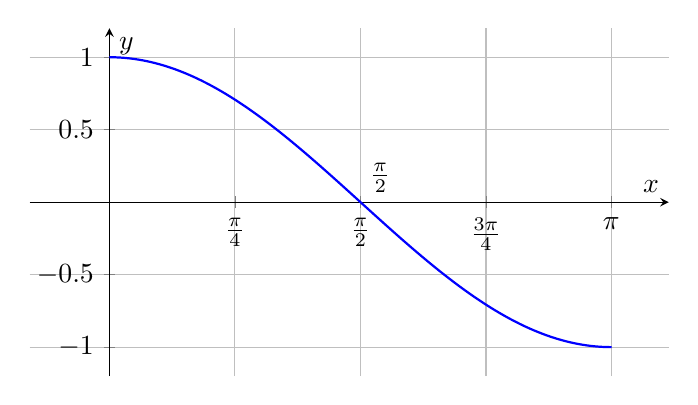
\begin{tikzpicture}
    \begin{axis}[
        width=0.8\linewidth,
        height=6cm,
        axis lines=middle,
        xlabel={$x$},
        ylabel={$y$},
        xmin=-0.5, xmax=3.5,
        ymin=-1.2, ymax=1.2,
        xtick={0, 0.785, 1.57, 2.356, 3.14},
        xticklabels={0, $\frac{\pi}{4}$, $\frac{\pi}{2}$, $\frac{3\pi}{4}$, $\pi$},
        ytick={-1, -0.5, 0, 0.5, 1},
        grid=both,
        samples=100
    ]
        \addplot[thick, blue, domain=0:3.14159] {cos(deg(x))};
        \node[above right] at (axis cs:1.57, 0) {$\frac{\pi}{2}$};
    \end{axis}
\end{tikzpicture}
\captionof{figure}{Graph of $y = \cos x$}
\end{center}

\textbf{Table of Key Points:}
\begin{center}
\begin{tabulary}{\linewidth}{|L|L|L|L|L|L|}
\hline
$x$ & $0$ & $\frac{\pi}{3}$ & $\frac{\pi}{2}$ & $\frac{2\pi}{3}$ & $\pi$ \\ \hline
$y = \cos x$ & $1$ & $0.5$ & $0$ & $-0.5$ & $-1$ \\ \hline
\end{tabulary}
\end{center}

\textbf{Properties:}
\begin{itemize}
    \item \textbf{Domain}: $[0, \pi]$
    \item \textbf{Range}: $[-1, 1]$ for full cycle, here max is 1, min is -1.
    \item \textbf{Zero}: at $x = \pi/2$
\end{itemize}
\end{solutionbox}

\questionmarks{3.2}{4}{Prove that $\tan^{-1}\frac{2}{3} + \tan^{-1}\frac{10}{11} + \tan^{-1}\frac{1}{4} = \frac{\pi}{2}$}
\begin{solutionbox}
\textbf{Solution}:
Let $A = \tan^{-1}\frac{2}{3}$, $B = \tan^{-1}\frac{10}{11}$.
Sum of first two using $\tan^{-1}x + \tan^{-1}y = \tan^{-1}\frac{x+y}{1-xy}$:
\[ \tan(A+B) = \frac{\frac{2}{3} + \frac{10}{11}}{1 - \frac{2}{3} \cdot \frac{10}{11}} = \frac{\frac{22+30}{33}}{1 - \frac{20}{33}} = \frac{\frac{52}{33}}{\frac{13}{33}} = \frac{52}{13} = 4 \]
So $A+B = \tan^{-1}(4)$.

Now add third term $\tan^{-1}\frac{1}{4}$:
\[ \tan^{-1}(4) + \tan^{-1}(\frac{1}{4}) \]
Since $\tan^{-1}x + \cot^{-1}x = \frac{\pi}{2}$ and $\tan^{-1}(\frac{1}{x}) = \cot^{-1}x$ for $x>0$:
\[ = \tan^{-1}(4) + \cot^{-1}(4) = \frac{\pi}{2} = \text{RHS} \]
\end{solutionbox}

\questionmarks{3.3}{4}{Find the unit vector perpendicular to both $5i + 7j - 2k$ and $i - 2j + 3k$}
\begin{solutionbox}
\textbf{Solution}:
Let $\vec{a} = (5, 7, -2)$ and $\vec{b} = (1, -2, 3)$.
Cross product $\vec{a} \times \vec{b}$ gives perpendicular vector.
\[ \vec{a} \times \vec{b} = \begin{vmatrix} \hat{i} & \hat{j} & \hat{k} \\ 5 & 7 & -2 \\ 1 & -2 & 3 \end{vmatrix} \]
\[ = \hat{i}(21 - 4) - \hat{j}(15 - (-2)) + \hat{k}(-10 - 7) \]
(Note: $7 \times 3 = 21$, $-2 \times -2 = 4$; $5 \times 3 = 15$, $-2 \times 1 = -2$)
\[ = \hat{i}(17) - \hat{j}(17) + \hat{k}(-17) = 17\hat{i} - 17\hat{j} - 17\hat{k} \]

Unit vector $\hat{n} = \frac{\vec{v}}{|\vec{v}|}$.
$|\vec{v}| = \sqrt{17^2 + (-17)^2 + (-17)^2} = \sqrt{3 \times 17^2} = 17\sqrt{3}$.
\[ \hat{n} = \frac{17(\hat{i} - \hat{j} - \hat{k})}{17\sqrt{3}} = \frac{\hat{i} - \hat{j} - \hat{k}}{\sqrt{3}} \]
\end{solutionbox}

\questionmarks{4(A)}{6}{Attempt any two}

\questionmarks{4.1}{3}{If $\vec{a} = i + 2j - k$, $\vec{b} = 3i - j + 2k$ and $\vec{c} = 2i - j + 5k$ then find $|2\vec{a} - 3\vec{b} + \vec{c}|$}
\begin{solutionbox}
\textbf{Solution}:
$2\vec{a} = 2i + 4j - 2k$
$-3\vec{b} = -9i + 3j - 6k$
$\vec{c} = 2i - j + 5k$

Sum $= (2 - 9 + 2)i + (4 + 3 - 1)j + (-2 - 6 + 5)k$
$= -5i + 6j - 3k$

Magnitude $= \sqrt{(-5)^2 + 6^2 + (-3)^2}$
$= \sqrt{25 + 36 + 9} = \sqrt{70}$
\end{solutionbox}

\questionmarks{4.2}{3}{Prove that the vectors $2i - 3j + k$ and $3i + j - 3k$ are perpendicular to each other}
\begin{solutionbox}
\textbf{Solution}:
Let $\vec{A} = (2, -3, 1)$ and $\vec{B} = (3, 1, -3)$.
Dot product $\vec{A} \cdot \vec{B} = (2)(3) + (-3)(1) + (1)(-3)$
$= 6 - 3 - 3 = 0$.
Since dot product is zero, vectors are perpendicular.
\end{solutionbox}

\questionmarks{4.3}{3}{Find the equation of line passing through point $(1,4)$ and having slope 6}
\begin{solutionbox}
\textbf{Solution}:
Point $(x_1, y_1) = (1, 4)$, Slope $m = 6$.
Equation: $y - 4 = 6(x - 1)$
\[ y - 4 = 6x - 6 \]
\[ 6x - y - 2 = 0 \]
\end{solutionbox}

\questionmarks{4(B)}{8}{Attempt any two}

\questionmarks{4.1}{4}{Prove that the angle between vectors $3i + j + 2k$ and $2i - 2j + 4k$ is $\sin^{-1}(\frac{2}{\sqrt{7}})$}
\begin{solutionbox}
\textbf{Solution}:
$\vec{A} = (3, 1, 2)$, $\vec{B} = (2, -2, 4)$.
$\vec{A} \cdot \vec{B} = 6 - 2 + 8 = 12$.
$|\vec{A}| = \sqrt{9+1+4} = \sqrt{14}$.
$|\vec{B}| = \sqrt{4+4+16} = \sqrt{24} = 2\sqrt{6}$.

$\cos\theta = \frac{12}{\sqrt{14} \cdot 2\sqrt{6}} = \frac{6}{\sqrt{84}} = \frac{6}{2\sqrt{21}} = \frac{3}{\sqrt{21}}$.

$\sin^2\theta = 1 - \cos^2\theta = 1 - \frac{9}{21} = 1 - \frac{3}{7} = \frac{4}{7}$.
$\sin\theta = \sqrt{\frac{4}{7}} = \frac{2}{\sqrt{7}}$.
$\theta = \sin^{-1}(\frac{2}{\sqrt{7}})$.
\end{solutionbox}

\questionmarks{4.2}{4}{A particle moves from point $(3,-2,1)$ to point $(1,3,-4)$ under the effect of constant forces $i - j + k$, $i + j - 3k$ and $4i + 5j - 6k$. Find the work done.}
\begin{solutionbox}
\textbf{Solution}:
Total Force $\vec{F} = (1+1+4)i + (-1+1+5)j + (1-3-6)k = 6i + 5j - 8k$.
Displacement $\vec{d} = \text{Final} - \text{Initial} = (1-3)i + (3-(-2))j + (-4-1)k = -2i + 5j - 5k$.

$W = \vec{F} \cdot \vec{d} = (6)(-2) + (5)(5) + (-8)(-5)$
$= -12 + 25 + 40 = 53$ units.
\end{solutionbox}

\questionmarks{4.3}{4}{Evaluate: (i) $\lim_{x \to 0} \frac{e^{2x} - 1}{x}$, (ii) $\lim_{x \to \infty} (1 + \frac{4}{x})^x$}
\begin{solutionbox}
\textbf{Solution}:
(i) $\lim_{x \to 0} \frac{e^{2x} - 1}{x}$.
Multiply/divide by 2:
$= 2 \lim_{2x \to 0} \frac{e^{2x} - 1}{2x} = 2(1) = 2$.

(ii) $\lim_{x \to \infty} (1 + \frac{4}{x})^x$.
Standard form $\lim_{x \to \infty} (1 + \frac{k}{x})^x = e^k$.
Here $k=4$, so Limit $= e^4$.
\end{solutionbox}

\questionmarks{5(A)}{6}{Attempt any two}

\questionmarks{5.1}{3}{Evaluate: $\lim_{x \to -2} \frac{x^2 + x - 6}{x^2 + 3x - 10}$}
\begin{solutionbox}
\textbf{Solution}:
At $x=-2$, form is $-4/-12$ (Wait, check math).
Numerator: $4 - 2 - 6 = -4 \neq 0$.
Denominator: $4 - 6 - 10 = -12 \neq 0$.
Wait, the MDX solution says "Since both are non-zero... = 1/3".
Wait, $4-2-6 = -4$? yes. $4-6-10 = -12$? yes.
So it is direct subs.
Result $= \frac{-4}{-12} = \frac{1}{3}$.
\end{solutionbox}

\questionmarks{5.2}{3}{Evaluate: $\lim_{x \to \infty} \frac{x^3 - 3x^2 + 2x - 1}{x(3x - 1)(2x + 1)}$}
\begin{solutionbox}
\textbf{Solution}:
Degree of numerator is 3. Degree of denominator is 3 ($x \cdot 3x \cdot 2x = 6x^3$).
Limit is ratio of leading coefficients.
Leading term Num: $1x^3$.
Leading term Denom: $6x^3$.
Limit $= \frac{1}{6}$.
\end{solutionbox}

\questionmarks{5.3}{3}{Evaluate: $\lim_{n \to \infty} \frac{1 + 2 + ... + n}{3n^2 - 2n - 4n^2}$}
\begin{solutionbox}
\textbf{Solution}:
Sum $= \frac{n(n+1)}{2} = \frac{n^2+n}{2}$.
Denominator $= 3n^2 - 4n^2 - 2n = -n^2 - 2n$.
Limit $= \lim_{n \to \infty} \frac{0.5n^2}{-1n^2} = -0.5 = -\frac{1}{2}$.
\end{solutionbox}

\questionmarks{5(B)}{8}{Attempt any two}

\questionmarks{5.1}{4}{Find the angle between two lines $\sqrt{3}x - y + 1 = 0$ and $x - \sqrt{3}y + 2 = 0$}
\begin{solutionbox}
\textbf{Solution}:
Line 1: $y = \sqrt{3}x + 1 \implies m_1 = \sqrt{3}$.
Line 2: $\sqrt{3}y = x + 2 \implies y = \frac{1}{\sqrt{3}}x + \dots \implies m_2 = \frac{1}{\sqrt{3}}$.

$\tan\theta = |\frac{m_1 - m_2}{1 + m_1 m_2}| = |\frac{\sqrt{3} - \frac{1}{\sqrt{3}}}{1 + \sqrt{3}(\frac{1}{\sqrt{3}})}| = |\frac{\frac{3-1}{\sqrt{3}}}{1+1}| = \frac{\frac{2}{\sqrt{3}}}{2} = \frac{1}{\sqrt{3}}$.
$\theta = \tan^{-1}\frac{1}{\sqrt{3}} = 30^\circ = \frac{\pi}{6}$.
\end{solutionbox}

\questionmarks{5.2}{4}{Find the center and radius of circle $4x^2 + 4y^2 + 8x - 12y - 3 = 0$}
\begin{solutionbox}
\textbf{Solution}:
Divide by 4:
$x^2 + y^2 + 2x - 3y - \frac{3}{4} = 0$.
$g = 1$, $f = -3/2$, $c = -3/4$.
Center $= (-g, -f) = (-1, \frac{3}{2})$.
Radius $= \sqrt{g^2 + f^2 - c} = \sqrt{1 + \frac{9}{4} + \frac{3}{4}} = \sqrt{1 + \frac{12}{4}} = \sqrt{1 + 3} = \sqrt{4} = 2$.
\end{solutionbox}

\questionmarks{5.3}{4}{Find the tangent and normal to circle $x^2 + y^2 - 4x + 2y + 3 = 0$ at point $(1, -2)$}
\begin{solutionbox}
\textbf{Solution}:
Center of circle: $2g = -4 \implies g=-2$, $2f=2 \implies f=1$. Center $C(2, -1)$.
Point $P(1, -2)$.
Slope of normal (Radius CP): $m_N = \frac{-2 - (-1)}{1 - 2} = \frac{-1}{-1} = 1$.
Equation of Normal: $y - (-2) = 1(x - 1) \implies y+2 = x-1 \implies x - y - 3 = 0$.

Slope of Tangent (perp to normal): $m_T = -1/m_N = -1$.
Equation of Tangent: $y - (-2) = -1(x - 1) \implies y+2 = -x+1 \implies x + y + 1 = 0$.
\end{solutionbox}

\section*{Formula Cheat Sheet}

\subsection*{Determinants}
\begin{itemize}
    \item $2 \times 2$: $ad - bc$
    \item Expansion Rules
\end{itemize}

\subsection*{Trigonometry}
\begin{itemize}
    \item $\tan(A+B) = \frac{\tan A + \tan B}{1 - \tan A \tan B}$
    \item $\tan 2A = \frac{2\tan A}{1 - \tan^2 A}$
    \item Angle between lines: $\tan\theta = |\frac{m_1 - m_2}{1 + m_1 m_2}|$
\end{itemize}

\subsection*{Limits}
\begin{itemize}
    \item $\lim_{x \to 0} \frac{e^x - 1}{x} = 1$
    \item $\lim_{x \to \infty} (1 + 1/x)^x = e$
\end{itemize}

\subsection*{Vectors}
\begin{itemize}
    \item Dot product $\vec{a} \cdot \vec{b} = |\vec{a}||\vec{b}|\cos\theta$
    \item Cross product for perpendicular vectors
\end{itemize}

\subsection*{Exponentials and Logarithms}
\begin{itemize}
    \item Change of base formula
    \item Logarithmic identities
\end{itemize}

\end{document}
